
Das Ziel des Visitor-Pattern ist, die Operationen auf Elemente in einer Objektstruktur außerhalb dieser Objektstruktur zu lagern um diese beliebig auszuwechseln.
Die Voraussetzung für jedes Element dieser Objektstruktur ist ein Interface \texttt{Element}, welches eine Methode \texttt{accept(Visitor)} erfordert. Dabei repräsentiert das übergebene Objekt \texttt{Visitor} die Operationen, die auf dieses Element angewendet werden sollen. Der Visitor selbst ist auch ein Interface. Das Interface muss für jeden Typ Element eine eigene Methode implementieren, die für die Bearbeitung der jeweiligen Elemente verantwortlich sind. Das bedeutet für unser UML-Diagramm, mit den zwei verschiedenen Elementen \texttt{ElementA} und \texttt{ElementB}, das wird zwei Methoden \texttt{visitElementA(ElementA)} und \texttt{visitElementB(ElementB)} definieren müssen. 
Der Ablauf des Visitor-Pattern ist folgendermaßen: Zunächst wird einem Element ein konkretes Visitor-Objekt übergeben. Dieses Element ruft dann die für sich implementierte Visit-Methode auf und übergibt sich selbst dem Visitor. Der Visitor kann dann auf das Element zugreifen und es bearbeiten.

\begin{figure}[htbp]
\centering
%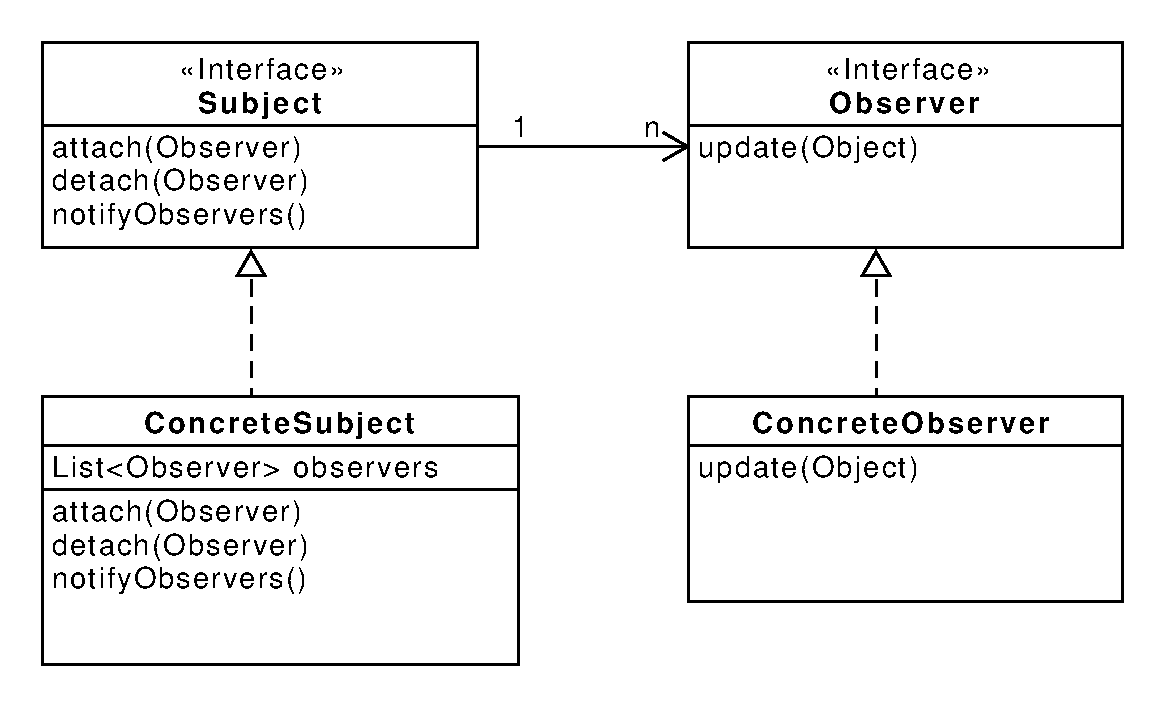
\includegraphics[scale=.5]{./observer/observer}
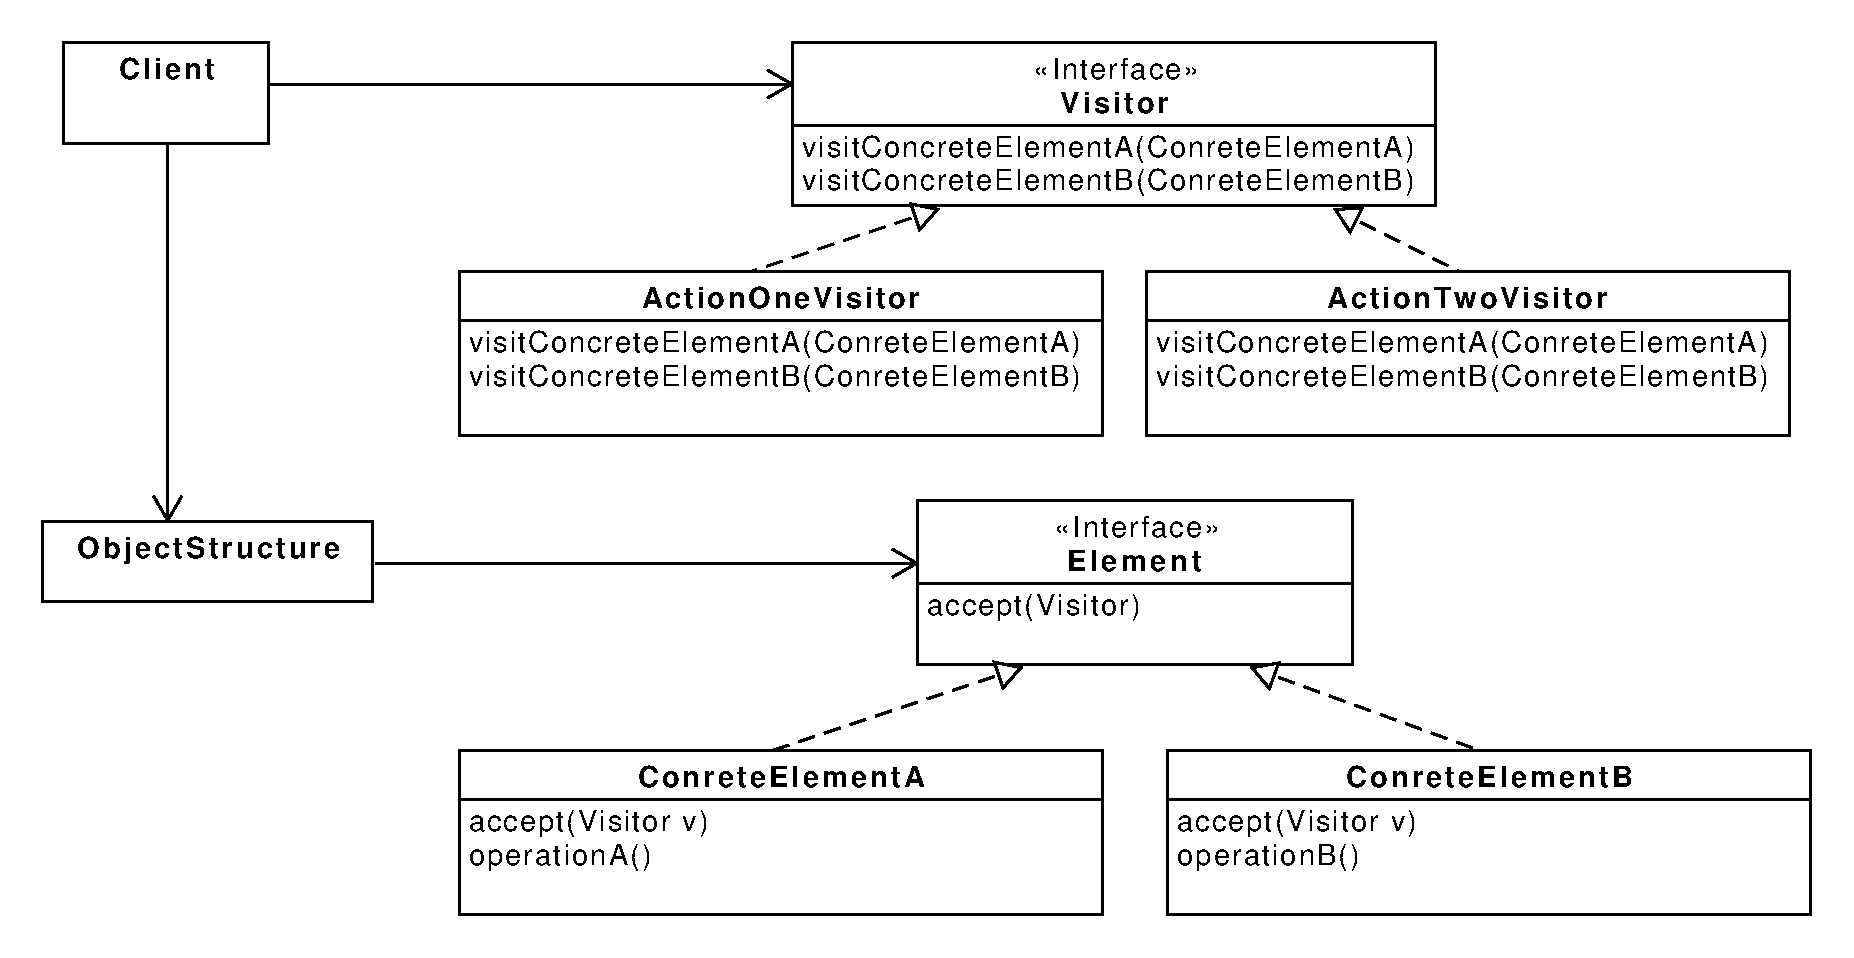
\includegraphics[width=0.7\textwidth]{./paper/visitor/visitor}
\caption{Eine UML-Darstellung von dem Visitor-Pattern.}
\label{visitordiagramm}
\end{figure} 
